\documentclass[12pt]{article}

\usepackage{amsmath}
\usepackage{amsfonts}
\usepackage{graphicx}
\usepackage{epstopdf}
\usepackage[margin=1in]{geometry}

\begin{document}

\section{Local Linear Regression}

Given the eigenvectors $\phi_1, \phi_2, \dots, \phi_{n-1} \in \mathbb{R}^n$, we would like to automatically deduce which ones are harmonics/functions of another. 
%
To accomplish this, we will fit a function $f(\phi_1, \dots, \phi_k)$ to $\phi_{k+1}$. 
%
If the resulting fit is good/accurate, then $\phi_{k+1}$ is most likely a harmonic of $\phi_1, \dots, \phi_k$. 

We will use a local linear function 
\begin{equation}
f_{k+1}(\phi_1, \dots, \phi_k) = a_0 + a_1 \phi_1 + \dots + a_k \phi_k
\end{equation}
where the coefficients $a_0, \dots, a_k$ are functions of $\phi_1, \dots, \phi_k$. 


To find these coefficients, we want to minimize the local weighted sum of squares
\begin{equation} \label{eq:opt_problem}
\sum_{i=1}^n w_i(x) (\phi_{k+1}(x) - f_{k+1} (\phi_1(x), \dots, \phi_{k}(x))
\end{equation}
where $w$ is a weighting function.
%
We will use
%
\begin{itemize}
\item $w_i(x) = \exp \left( - \frac{\|\Phi_{k}(x) - \Phi_{k} (x_i) \|^2}{\epsilon^2} \right)$, where $\Phi_k(x) = \begin{bmatrix}
\phi_1(x) \\
\vdots \\
\phi_k(x)
\end{bmatrix} $
\item $\epsilon = M / 3$, where $M$ is the median of the pairwise distances between $\Phi_{k}(x)$
\end{itemize}

Let $\hat{f}_{k+1}(\phi_1(x_i), \dots, \phi_k(x_i))$ denote the minimum achieved in \eqref{eq:opt_problem}, when the minimization is performed over $x_j$ with $j \ne i$. 
%
We then define the leave-one-out- cross-validation error as
\begin{equation}
r_{k+1} = \sum_{i=1}^n \left( \phi_{k+1} (x_i) - \hat{f}_{k+1}(\phi_1(x_i), \dots, \phi_k(x_i)) \right)^2
\end{equation}
%
A small value of $r_{k+1}$ means that $\phi_{k+1}$ can be accurately approximated from $\phi_1, \dots, \phi_k$, and is therefore a harmonic of a previous mode.
%
A large value of $r_{k+1}$ indicates that $\phi_{k+1}$ parameterizes a new direction in the data.

\section{Eigenvalues}

The eigenvalues of the Laplacian with Neumann boundary conditions on a $d$-dimensional rectangular domain are given by
\begin{equation}
\mu_{k,l} = \frac{k^2 \pi^2}{L_l^2}
\end{equation}
for $k=1, 2, \dots$ and $l=1, 2, \dots, d$, and $L_l$ is the length of the domain along the $l^{th}$ dimension. 
%
These eigenvalues are related to the eigenvalues we compute in diffusion maps by 
\begin{equation}
\lambda_{k,l} = e^{-\mu_{k,l} t} = e^{-\frac{k^2 \pi^2}{L_l^2} t}
\end{equation}
%
Therefore, 
\begin{equation}
\sqrt{\frac{\log(\lambda_{1,l_1})}{\log(\lambda_{1,l_2})}} = 
\frac{L_{l_2}}{L_{l_1}}
\end{equation}
and so looking at the ratio of the log of the eigenvalues (modulo harmonics) should inform us as to the lengths of the different directions in the manifold. 

\section{Example: Swiss Roll}

\centering
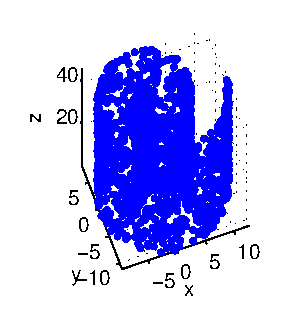
\includegraphics[height=3in]{swissroll1}
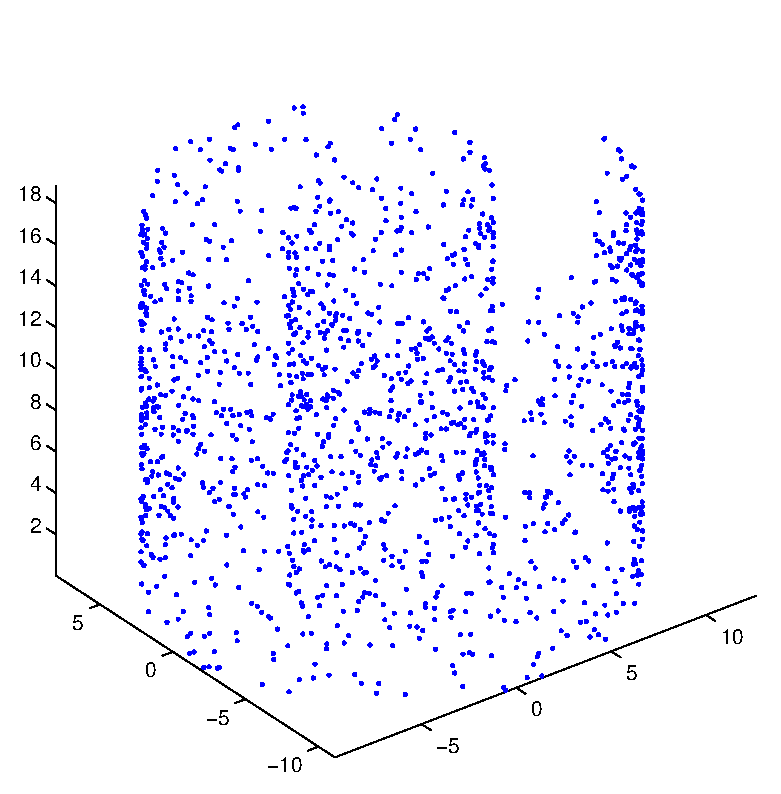
\includegraphics[height=3in]{swissroll2}\\
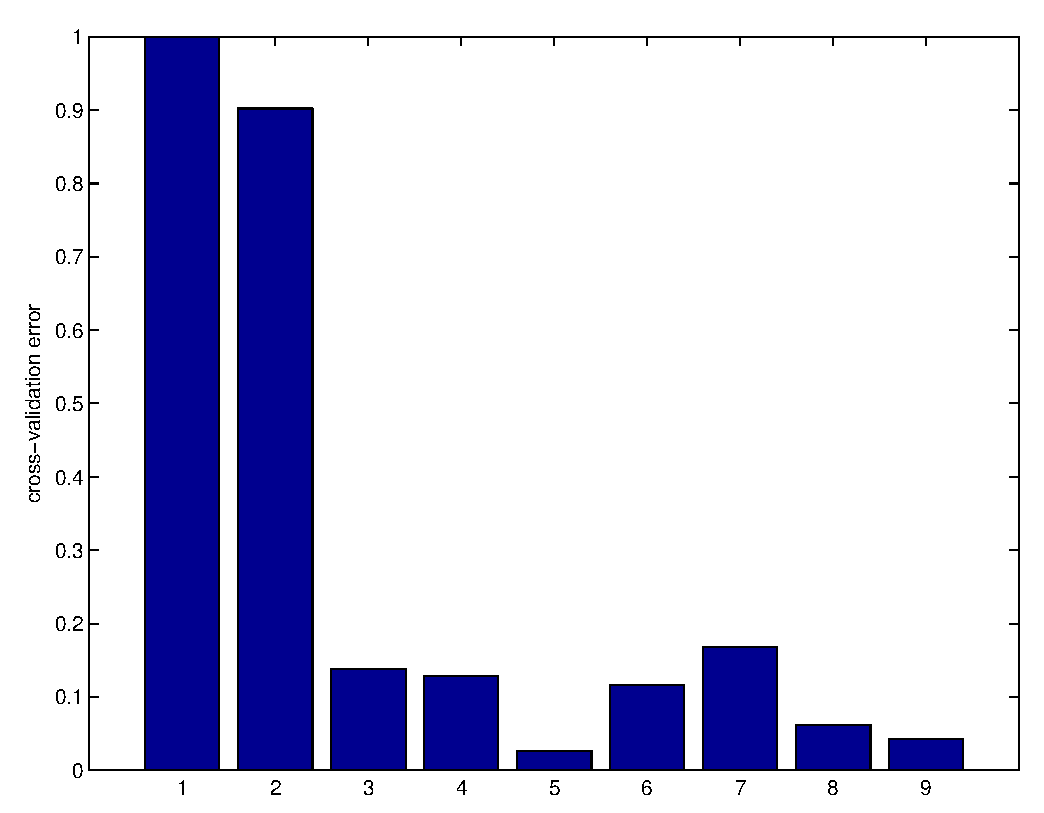
\includegraphics[height=2in]{swissroll1_cv}
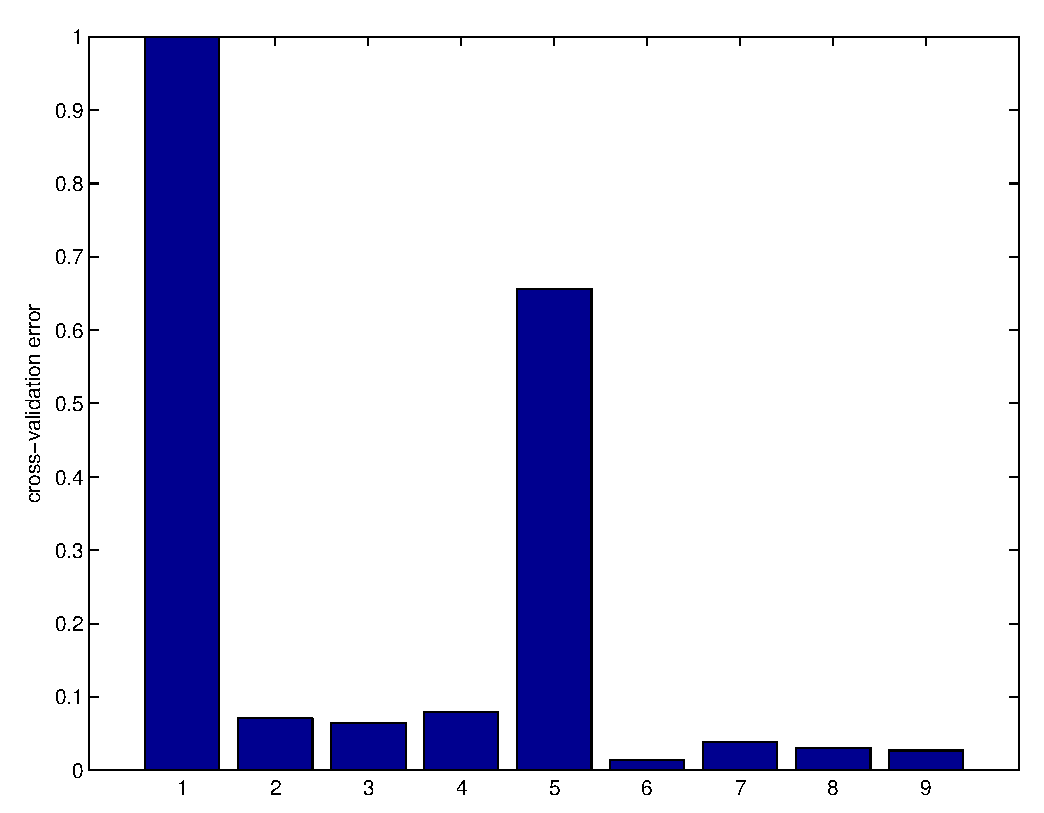
\includegraphics[height=2in]{swissroll2_cv}\\
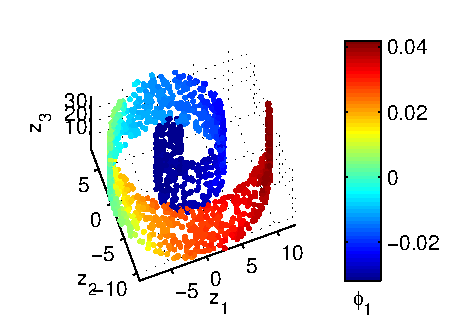
\includegraphics[height=3in]{swissroll1_color1}
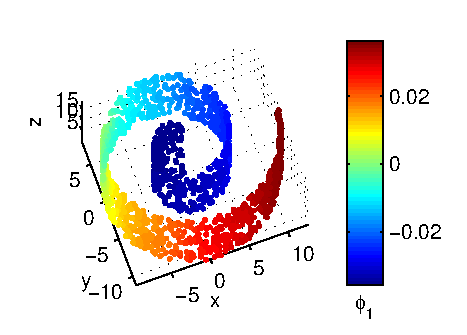
\includegraphics[height=3in]{swissroll2_color1}\\
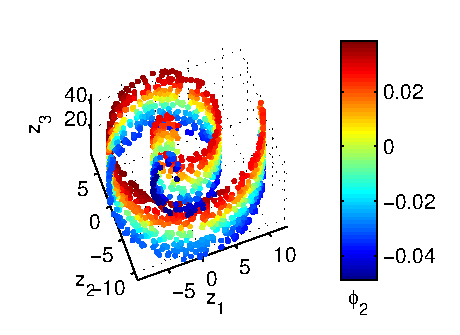
\includegraphics[height=3in]{swissroll1_color2}
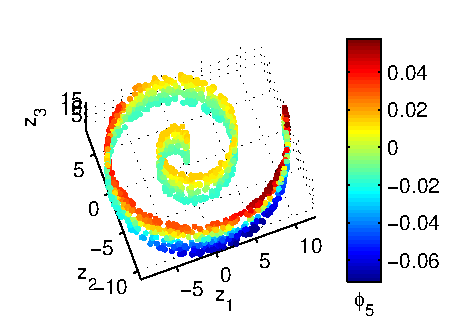
\includegraphics[height=3in]{swissroll2_color2}

For first case: $\lambda_1 = 0.9982$, $\lambda_2 = 0.9959$

For second case: $\lambda_1 = 0.9977$, $\lambda_5 = 0.9652$.

\section{Example: Chemotaxis Data}

\centering
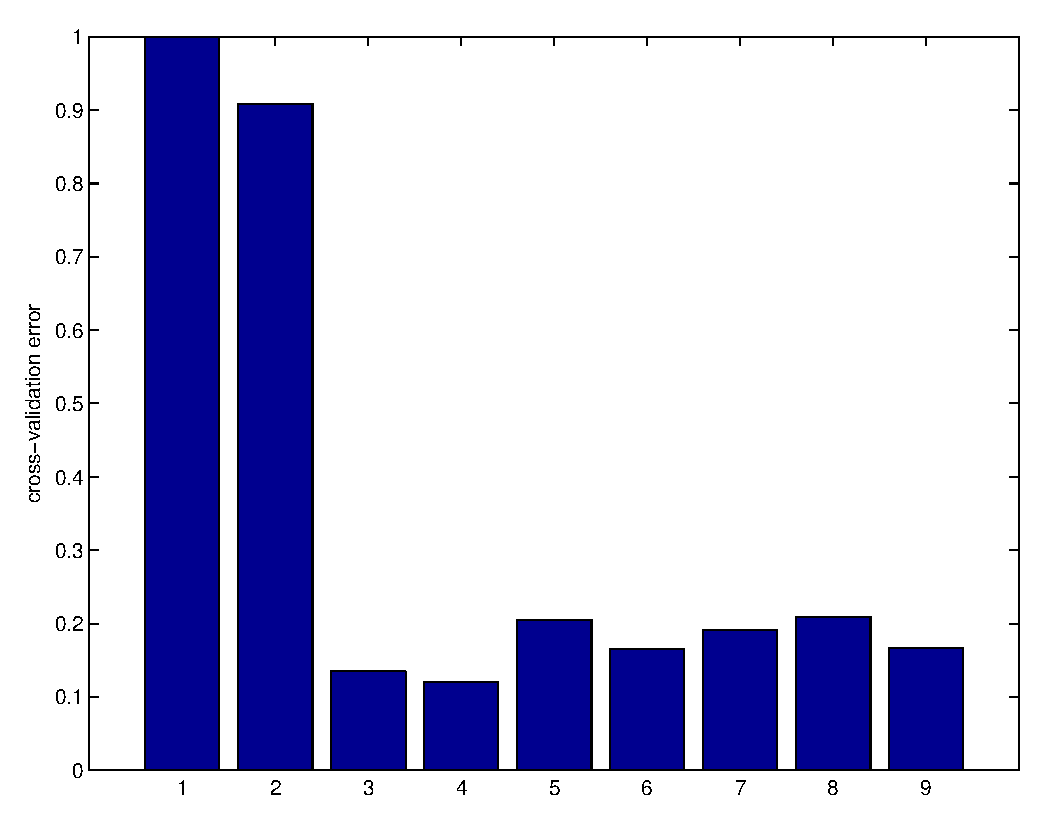
\includegraphics[height=2in]{lle_errors1}
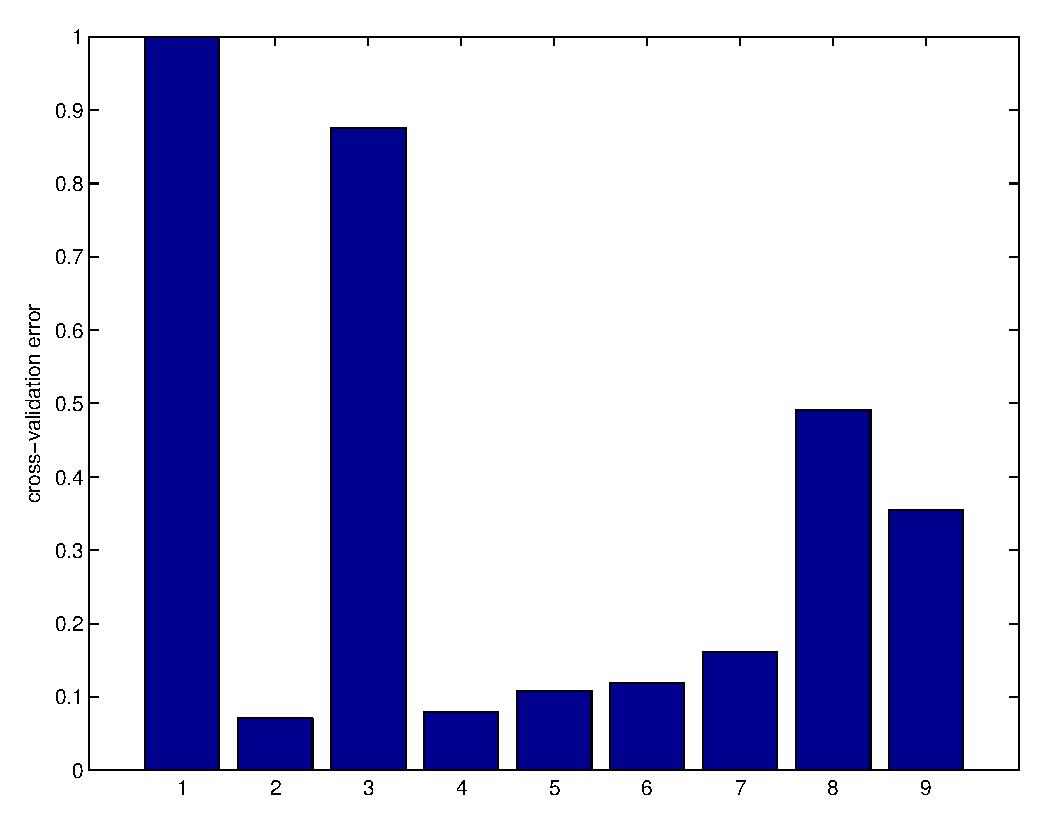
\includegraphics[height=2in]{lle_errors2}

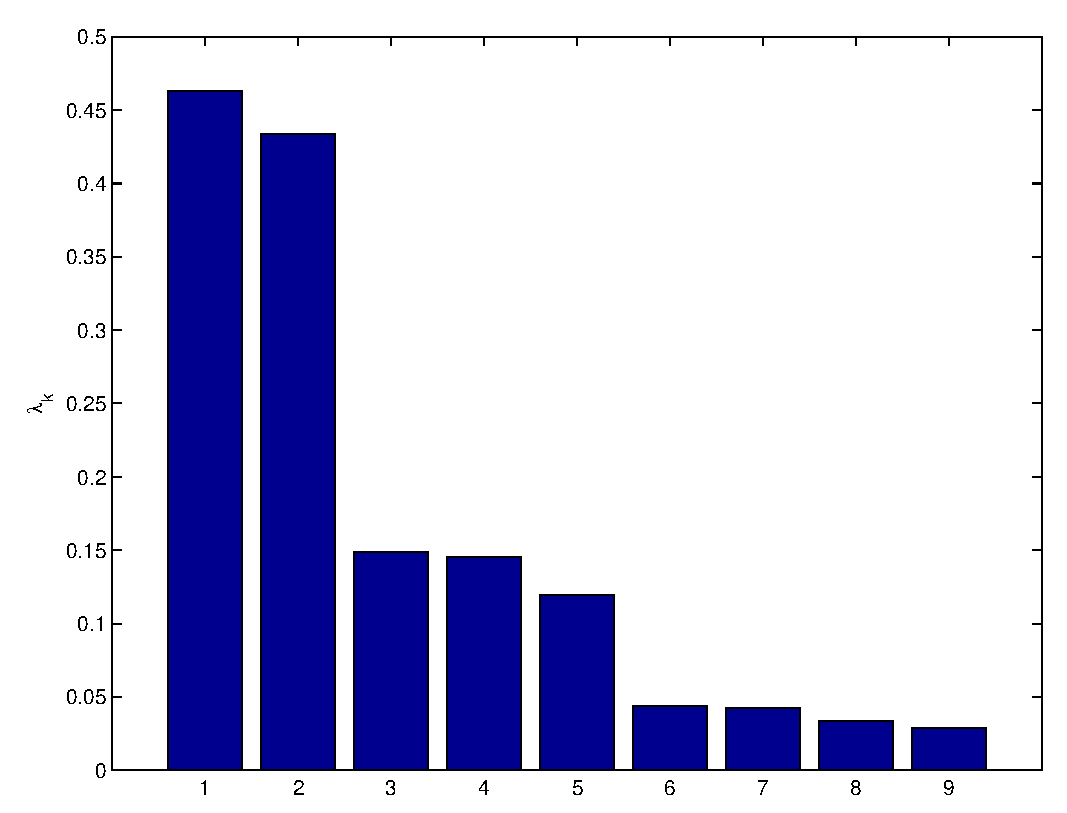
\includegraphics[height=2in]{lle_evals1}
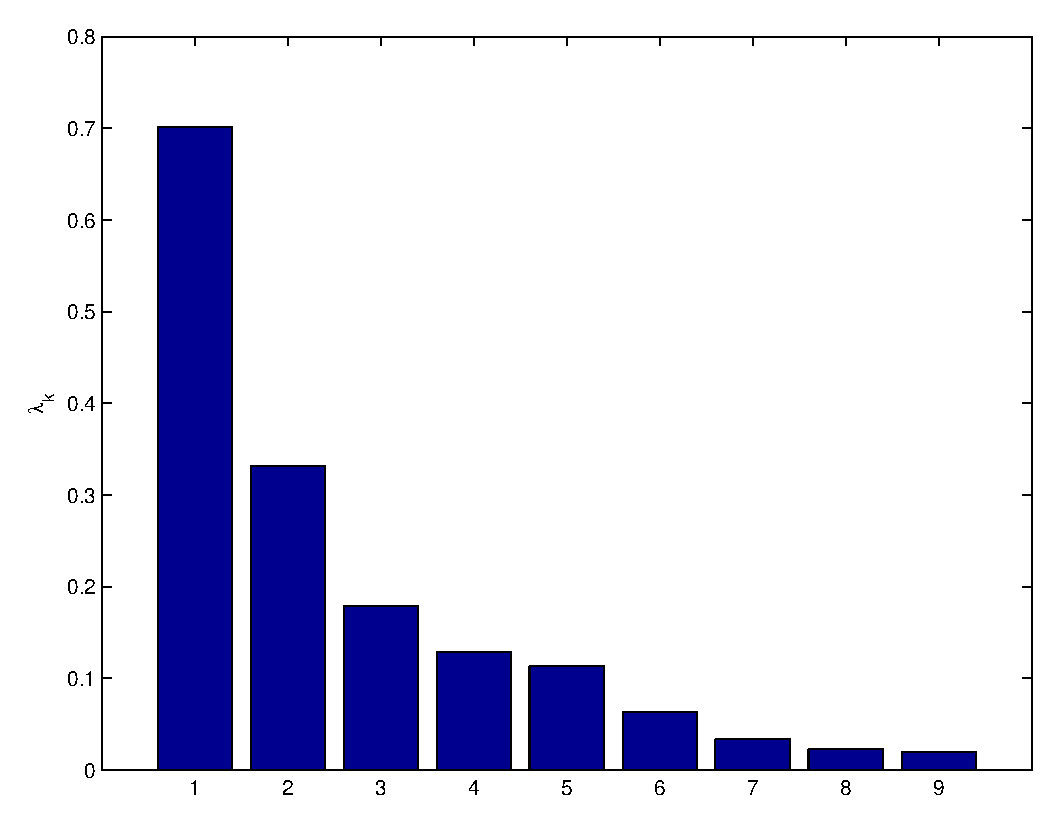
\includegraphics[height=2in]{lle_evals2}

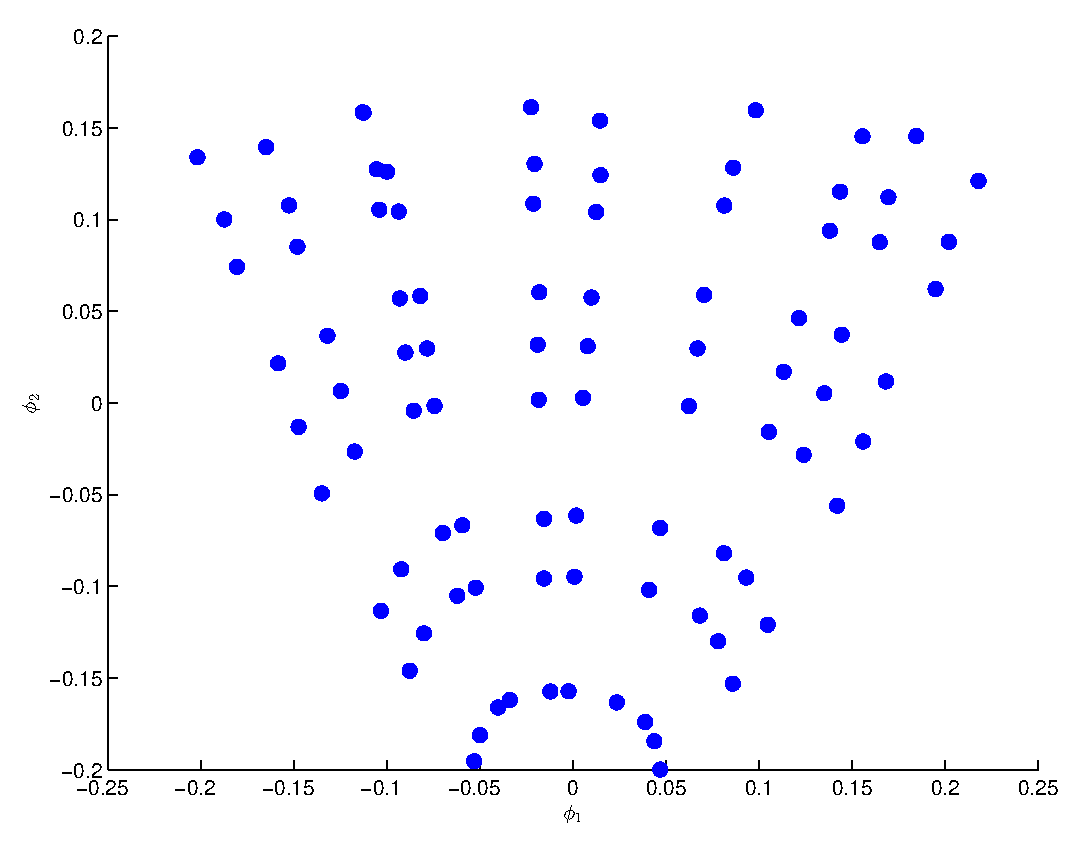
\includegraphics[height=2in]{lle_embed1_1}
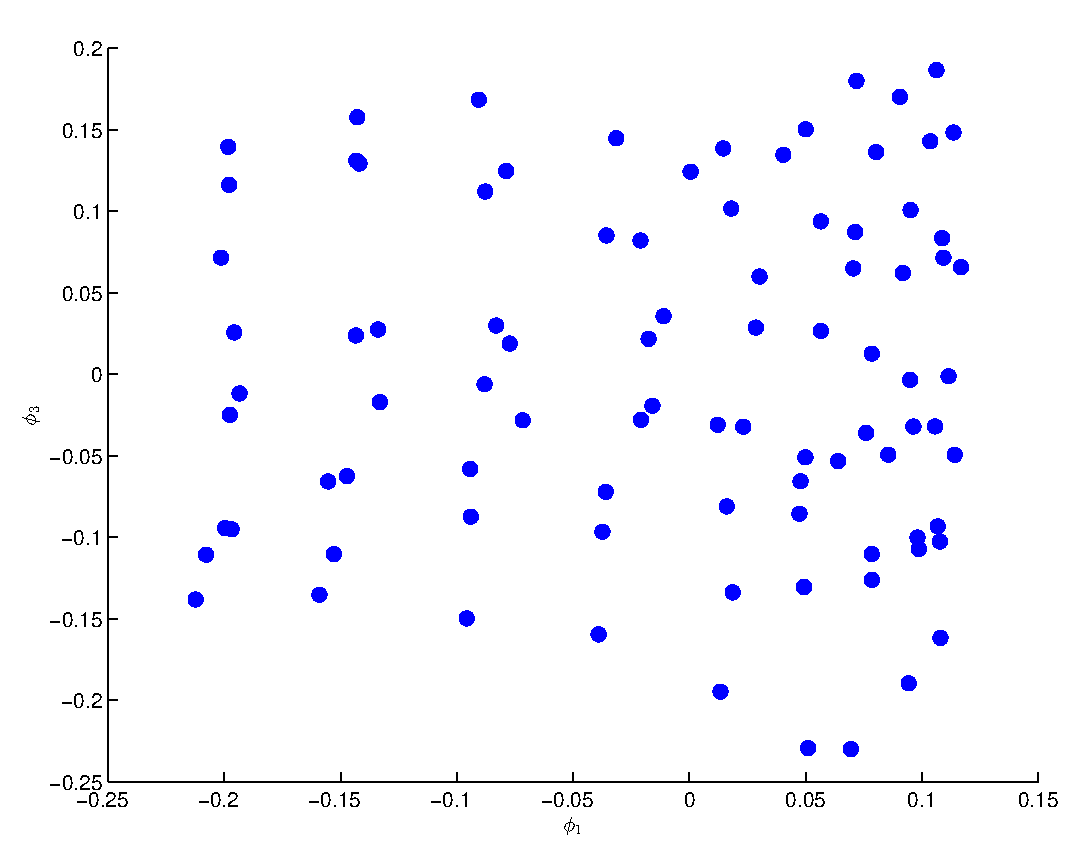
\includegraphics[height=2in]{lle_embed2_2}

\hfill 
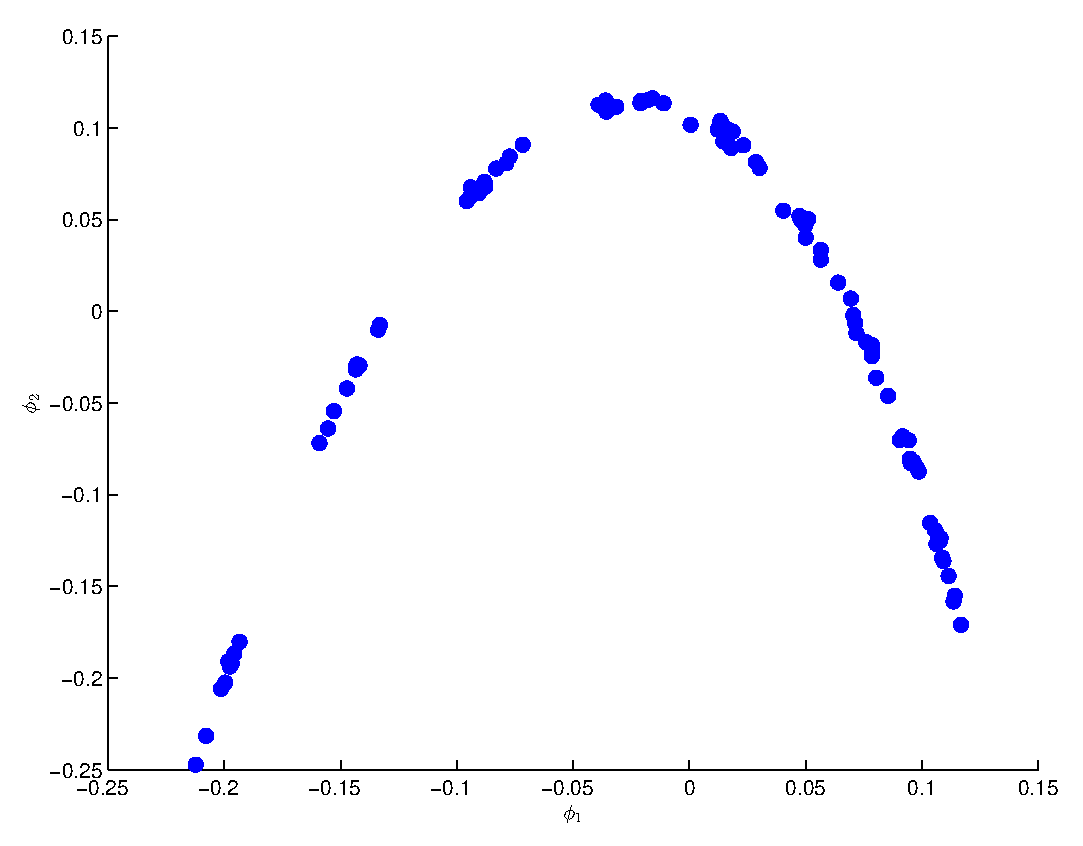
\includegraphics[height=2in]{lle_embed1_2}

\end{document}